\cajota{Población por sexo, según grupos de edad}{Para el 2022, el grupo de edad de 15 a 19 años tiene la población más grande de los grupos de edad con 956,598.8 miles de personas. El siguiente grupo más poblado es de 0 a 4 años de edad con 1681.9 miles de personas. Por el contrario,  la población de 100 años o más cuenta con la menor cantidad de personas de todos los grupos con 1.2 miles de personas. }{Población por sexo, según grupos de edad}{República de Guatemala, Instituto Nacional de Estadística -INE-, en miles de personas}{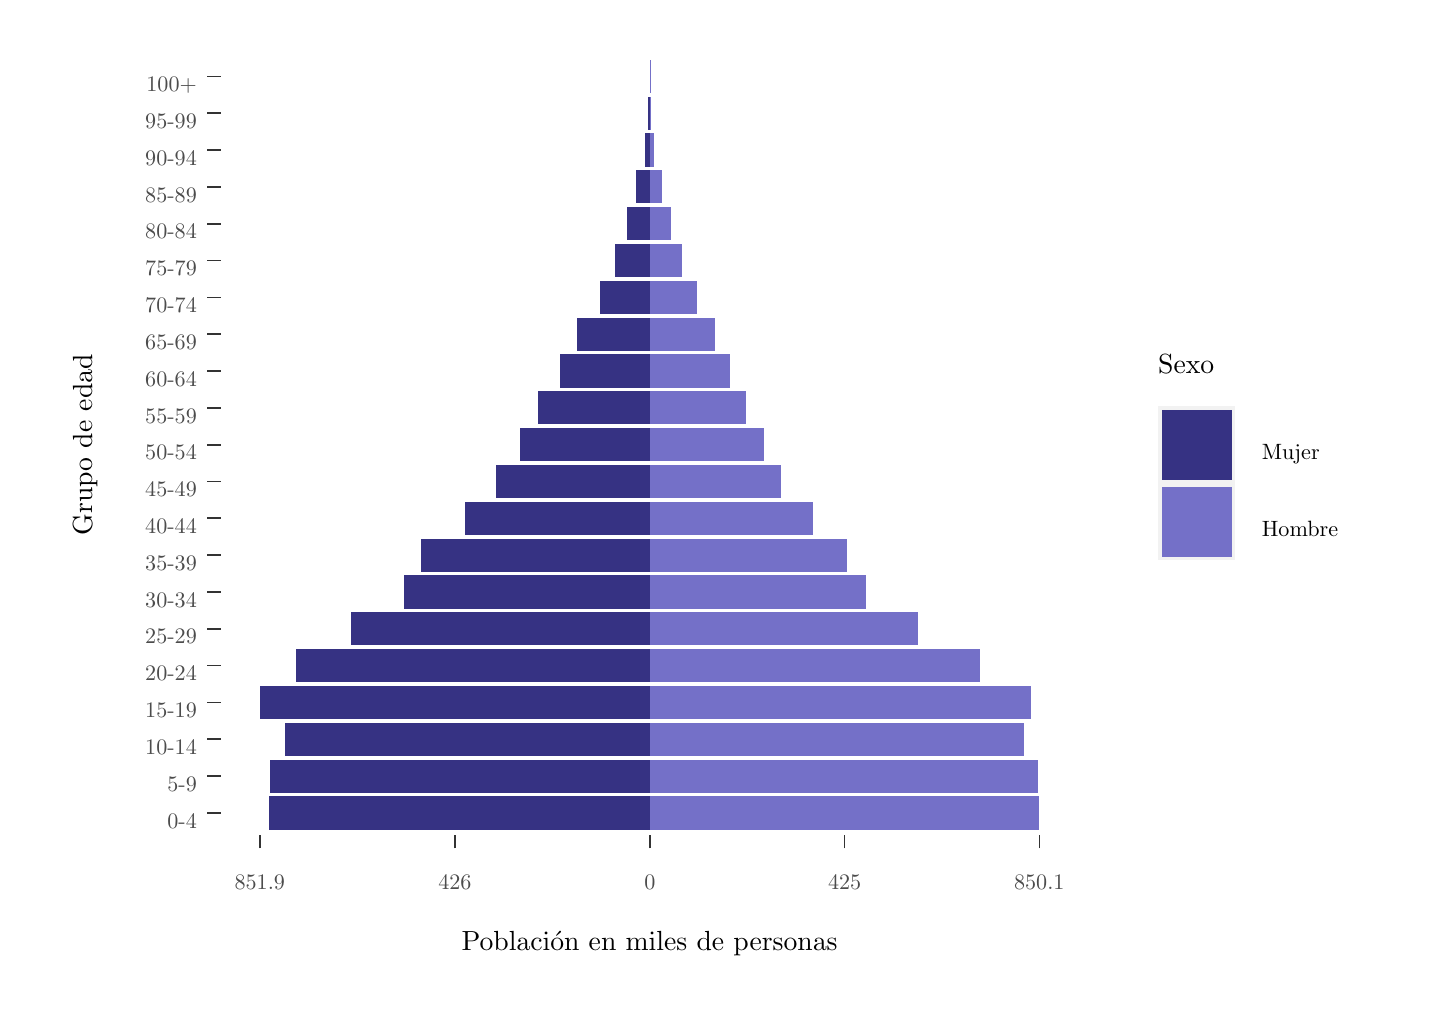
\begin{tikzpicture}[x=1pt,y=1pt, scale=1.75]% Created by tikzDevice version 0.12.4 on 2023-04-04 13:49:55
% !TEX encoding = UTF-8 Unicode
\definecolor{fillColor}{RGB}{255,255,255}
\path[use as bounding box,fill=fillColor,fill opacity=0.00] (0,0) rectangle (289.08,198.74);
\begin{scope}
\path[clip] (  0.00,  0.00) rectangle (289.08,198.74);
\definecolor{drawColor}{RGB}{255,255,255}
\definecolor{fillColor}{RGB}{255,255,255}

\path[draw=drawColor,line width= 0.6pt,line join=round,line cap=round,fill=fillColor] (  0.00,  0.00) rectangle (289.08,198.74);
\end{scope}
\begin{scope}
\path[clip] (  0.00,  0.00) rectangle (289.08,198.74);
\definecolor{fillColor}{RGB}{54,50,131}

\path[fill=fillColor] ( 49.83, 33.17) rectangle (128.50, 40.01);

\path[fill=fillColor] ( 50.06, 40.77) rectangle (128.50, 47.62);

\path[fill=fillColor] ( 53.08, 48.38) rectangle (128.50, 55.22);

\path[fill=fillColor] ( 47.93, 55.98) rectangle (128.50, 62.83);

\path[fill=fillColor] ( 55.37, 63.59) rectangle (128.50, 70.43);

\path[fill=fillColor] ( 66.82, 71.19) rectangle (128.50, 78.03);

\path[fill=fillColor] ( 77.71, 78.79) rectangle (128.50, 85.64);

\path[fill=fillColor] ( 81.13, 86.40) rectangle (128.50, 93.24);

\path[fill=fillColor] ( 90.24, 94.00) rectangle (128.50,100.85);

\path[fill=fillColor] ( 96.76,101.61) rectangle (128.50,108.45);

\path[fill=fillColor] (101.65,109.21) rectangle (128.50,116.06);

\path[fill=fillColor] (105.47,116.82) rectangle (128.50,123.66);

\path[fill=fillColor] (109.95,124.42) rectangle (128.50,131.27);

\path[fill=fillColor] (113.42,132.03) rectangle (128.50,138.87);

\path[fill=fillColor] (118.19,139.63) rectangle (128.50,146.47);

\path[fill=fillColor] (121.23,147.24) rectangle (128.50,154.08);

\path[fill=fillColor] (123.82,154.84) rectangle (128.50,161.68);

\path[fill=fillColor] (125.59,162.44) rectangle (128.50,169.29);

\path[fill=fillColor] (127.43,170.05) rectangle (128.50,176.89);

\path[fill=fillColor] (128.15,177.65) rectangle (128.50,184.50);

\path[fill=fillColor] (128.43,185.26) rectangle (128.50,192.10);
\definecolor{fillColor}{RGB}{116,112,200}

\path[fill=fillColor] (128.50, 33.17) rectangle (208.89, 40.01);

\path[fill=fillColor] (128.50, 40.77) rectangle (208.64, 47.62);

\path[fill=fillColor] (128.50, 48.38) rectangle (205.73, 55.22);

\path[fill=fillColor] (128.50, 55.98) rectangle (207.08, 62.83);

\path[fill=fillColor] (128.50, 63.59) rectangle (196.62, 70.43);

\path[fill=fillColor] (128.50, 71.19) rectangle (183.82, 78.03);

\path[fill=fillColor] (128.50, 78.79) rectangle (173.20, 85.64);

\path[fill=fillColor] (128.50, 86.40) rectangle (169.09, 93.24);

\path[fill=fillColor] (128.50, 94.00) rectangle (162.08,100.85);

\path[fill=fillColor] (128.50,101.61) rectangle (155.53,108.45);

\path[fill=fillColor] (128.50,109.21) rectangle (152.06,116.06);

\path[fill=fillColor] (128.50,116.82) rectangle (148.32,123.66);

\path[fill=fillColor] (128.50,124.42) rectangle (145.04,131.27);

\path[fill=fillColor] (128.50,132.03) rectangle (141.84,138.87);

\path[fill=fillColor] (128.50,139.63) rectangle (138.12,146.47);

\path[fill=fillColor] (128.50,147.24) rectangle (135.12,154.08);

\path[fill=fillColor] (128.50,154.84) rectangle (132.74,161.68);

\path[fill=fillColor] (128.50,162.44) rectangle (130.97,169.29);

\path[fill=fillColor] (128.50,170.05) rectangle (129.36,176.89);

\path[fill=fillColor] (128.50,177.65) rectangle (128.75,184.50);

\path[fill=fillColor] (128.50,185.26) rectangle (128.54,192.10);
\end{scope}
\begin{scope}
\path[clip] (  0.00,  0.00) rectangle (289.08,198.74);
\definecolor{drawColor}{gray}{0.30}

\node[text=drawColor,anchor=base east,inner sep=0pt, outer sep=0pt, scale=  0.80] at ( 34.93, 33.46) {0-4};

\node[text=drawColor,anchor=base east,inner sep=0pt, outer sep=0pt, scale=  0.80] at ( 34.93, 41.07) {5-9};

\node[text=drawColor,anchor=base east,inner sep=0pt, outer sep=0pt, scale=  0.80] at ( 34.93, 48.67) {10-14};

\node[text=drawColor,anchor=base east,inner sep=0pt, outer sep=0pt, scale=  0.80] at ( 34.93, 56.28) {15-19};

\node[text=drawColor,anchor=base east,inner sep=0pt, outer sep=0pt, scale=  0.80] at ( 34.93, 63.88) {20-24};

\node[text=drawColor,anchor=base east,inner sep=0pt, outer sep=0pt, scale=  0.80] at ( 34.93, 71.49) {25-29};

\node[text=drawColor,anchor=base east,inner sep=0pt, outer sep=0pt, scale=  0.80] at ( 34.93, 79.09) {30-34};

\node[text=drawColor,anchor=base east,inner sep=0pt, outer sep=0pt, scale=  0.80] at ( 34.93, 86.69) {35-39};

\node[text=drawColor,anchor=base east,inner sep=0pt, outer sep=0pt, scale=  0.80] at ( 34.93, 94.30) {40-44};

\node[text=drawColor,anchor=base east,inner sep=0pt, outer sep=0pt, scale=  0.80] at ( 34.93,101.90) {45-49};

\node[text=drawColor,anchor=base east,inner sep=0pt, outer sep=0pt, scale=  0.80] at ( 34.93,109.51) {50-54};

\node[text=drawColor,anchor=base east,inner sep=0pt, outer sep=0pt, scale=  0.80] at ( 34.93,117.11) {55-59};

\node[text=drawColor,anchor=base east,inner sep=0pt, outer sep=0pt, scale=  0.80] at ( 34.93,124.72) {60-64};

\node[text=drawColor,anchor=base east,inner sep=0pt, outer sep=0pt, scale=  0.80] at ( 34.93,132.32) {65-69};

\node[text=drawColor,anchor=base east,inner sep=0pt, outer sep=0pt, scale=  0.80] at ( 34.93,139.93) {70-74};

\node[text=drawColor,anchor=base east,inner sep=0pt, outer sep=0pt, scale=  0.80] at ( 34.93,147.53) {75-79};

\node[text=drawColor,anchor=base east,inner sep=0pt, outer sep=0pt, scale=  0.80] at ( 34.93,155.14) {80-84};

\node[text=drawColor,anchor=base east,inner sep=0pt, outer sep=0pt, scale=  0.80] at ( 34.93,162.74) {85-89};

\node[text=drawColor,anchor=base east,inner sep=0pt, outer sep=0pt, scale=  0.80] at ( 34.93,170.34) {90-94};

\node[text=drawColor,anchor=base east,inner sep=0pt, outer sep=0pt, scale=  0.80] at ( 34.93,177.95) {95-99};

\node[text=drawColor,anchor=base east,inner sep=0pt, outer sep=0pt, scale=  0.80] at ( 34.93,185.55) {100+};
\end{scope}
\begin{scope}
\path[clip] (  0.00,  0.00) rectangle (289.08,198.74);
\definecolor{drawColor}{gray}{0.20}

\path[draw=drawColor,line width= 0.6pt,line join=round] ( 37.13, 36.59) --
	( 39.88, 36.59);

\path[draw=drawColor,line width= 0.6pt,line join=round] ( 37.13, 44.19) --
	( 39.88, 44.19);

\path[draw=drawColor,line width= 0.6pt,line join=round] ( 37.13, 51.80) --
	( 39.88, 51.80);

\path[draw=drawColor,line width= 0.6pt,line join=round] ( 37.13, 59.40) --
	( 39.88, 59.40);

\path[draw=drawColor,line width= 0.6pt,line join=round] ( 37.13, 67.01) --
	( 39.88, 67.01);

\path[draw=drawColor,line width= 0.6pt,line join=round] ( 37.13, 74.61) --
	( 39.88, 74.61);

\path[draw=drawColor,line width= 0.6pt,line join=round] ( 37.13, 82.22) --
	( 39.88, 82.22);

\path[draw=drawColor,line width= 0.6pt,line join=round] ( 37.13, 89.82) --
	( 39.88, 89.82);

\path[draw=drawColor,line width= 0.6pt,line join=round] ( 37.13, 97.43) --
	( 39.88, 97.43);

\path[draw=drawColor,line width= 0.6pt,line join=round] ( 37.13,105.03) --
	( 39.88,105.03);

\path[draw=drawColor,line width= 0.6pt,line join=round] ( 37.13,112.63) --
	( 39.88,112.63);

\path[draw=drawColor,line width= 0.6pt,line join=round] ( 37.13,120.24) --
	( 39.88,120.24);

\path[draw=drawColor,line width= 0.6pt,line join=round] ( 37.13,127.84) --
	( 39.88,127.84);

\path[draw=drawColor,line width= 0.6pt,line join=round] ( 37.13,135.45) --
	( 39.88,135.45);

\path[draw=drawColor,line width= 0.6pt,line join=round] ( 37.13,143.05) --
	( 39.88,143.05);

\path[draw=drawColor,line width= 0.6pt,line join=round] ( 37.13,150.66) --
	( 39.88,150.66);

\path[draw=drawColor,line width= 0.6pt,line join=round] ( 37.13,158.26) --
	( 39.88,158.26);

\path[draw=drawColor,line width= 0.6pt,line join=round] ( 37.13,165.87) --
	( 39.88,165.87);

\path[draw=drawColor,line width= 0.6pt,line join=round] ( 37.13,173.47) --
	( 39.88,173.47);

\path[draw=drawColor,line width= 0.6pt,line join=round] ( 37.13,181.08) --
	( 39.88,181.08);

\path[draw=drawColor,line width= 0.6pt,line join=round] ( 37.13,188.68) --
	( 39.88,188.68);
\end{scope}
\begin{scope}
\path[clip] (  0.00,  0.00) rectangle (289.08,198.74);
\definecolor{drawColor}{gray}{0.20}

\path[draw=drawColor,line width= 0.6pt,line join=round] ( 47.93, 29.28) --
	( 47.93, 32.03);

\path[draw=drawColor,line width= 0.6pt,line join=round] ( 88.21, 29.28) --
	( 88.21, 32.03);

\path[draw=drawColor,line width= 0.6pt,line join=round] (128.50, 29.28) --
	(128.50, 32.03);

\path[draw=drawColor,line width= 0.6pt,line join=round] (168.69, 29.28) --
	(168.69, 32.03);

\path[draw=drawColor,line width= 0.6pt,line join=round] (208.89, 29.28) --
	(208.89, 32.03);
\end{scope}
\begin{scope}
\path[clip] (  0.00,  0.00) rectangle (289.08,198.74);
\definecolor{drawColor}{gray}{0.30}

\node[text=drawColor,anchor=base,inner sep=0pt, outer sep=0pt, scale=  0.80] at ( 47.93, 20.82) {851.9};

\node[text=drawColor,anchor=base,inner sep=0pt, outer sep=0pt, scale=  0.80] at ( 88.21, 20.82) {426};

\node[text=drawColor,anchor=base,inner sep=0pt, outer sep=0pt, scale=  0.80] at (128.50, 20.82) {0};

\node[text=drawColor,anchor=base,inner sep=0pt, outer sep=0pt, scale=  0.80] at (168.69, 20.82) {425};

\node[text=drawColor,anchor=base,inner sep=0pt, outer sep=0pt, scale=  0.80] at (208.89, 20.82) {850.1};
\end{scope}
\begin{scope}
\path[clip] (  0.00,  0.00) rectangle (289.08,198.74);
\definecolor{drawColor}{RGB}{0,0,0}

\node[text=drawColor,anchor=base,inner sep=0pt, outer sep=0pt, scale=  1.00] at (128.41,  8.14) {Población en miles de personas};
\end{scope}
\begin{scope}
\path[clip] (  0.00,  0.00) rectangle (289.08,198.74);
\definecolor{drawColor}{RGB}{0,0,0}

\node[text=drawColor,rotate= 90.00,anchor=base,inner sep=0pt, outer sep=0pt, scale=  1.00] at ( 13.32,112.63) {Grupo de edad};
\end{scope}
\begin{scope}
\path[clip] (  0.00,  0.00) rectangle (289.08,198.74);
\definecolor{fillColor}{RGB}{255,255,255}

\path[fill=fillColor] (227.94, 83.26) rectangle (283.58,142.01);
\end{scope}
\begin{scope}
\path[clip] (  0.00,  0.00) rectangle (289.08,198.74);
\definecolor{drawColor}{RGB}{0,0,0}

\node[text=drawColor,anchor=base west,inner sep=0pt, outer sep=0pt, scale=  1.00] at (233.44,127.38) {Sexo};
\end{scope}
\begin{scope}
\path[clip] (  0.00,  0.00) rectangle (289.08,198.74);
\definecolor{fillColor}{gray}{0.95}

\path[fill=fillColor] (233.44,104.66) rectangle (249.34,120.55);
\end{scope}
\begin{scope}
\path[clip] (  0.00,  0.00) rectangle (289.08,198.74);
\definecolor{fillColor}{RGB}{54,50,131}

\path[fill=fillColor] (234.15,105.37) rectangle (248.63,119.84);
\end{scope}
\begin{scope}
\path[clip] (  0.00,  0.00) rectangle (289.08,198.74);
\definecolor{fillColor}{gray}{0.95}

\path[fill=fillColor] (233.44, 88.76) rectangle (249.34,104.66);
\end{scope}
\begin{scope}
\path[clip] (  0.00,  0.00) rectangle (289.08,198.74);
\definecolor{fillColor}{RGB}{116,112,200}

\path[fill=fillColor] (234.15, 89.47) rectangle (248.63,103.94);
\end{scope}
\begin{scope}
\path[clip] (  0.00,  0.00) rectangle (289.08,198.74);
\definecolor{drawColor}{RGB}{0,0,0}

\node[text=drawColor,anchor=base west,inner sep=0pt, outer sep=0pt, scale=  0.80] at (254.84,109.48) {Mujer};
\end{scope}
\begin{scope}
\path[clip] (  0.00,  0.00) rectangle (289.08,198.74);
\definecolor{drawColor}{RGB}{0,0,0}

\node[text=drawColor,anchor=base west,inner sep=0pt, outer sep=0pt, scale=  0.80] at (254.84, 93.58) {Hombre};
\end{scope}
\end{tikzpicture}}{INE - Censo 2018}

\cajita{Población por sexo, según dominio de estudio}{Para 2022, según las proyecciones de población del Instituto Nacional de Estadística, en la República de Guatemala habitaban 17,357,886 personas. }{Población por sexo, según dominio de estudio}{República de Guatemala, Instituto Nacional de Estadística -INE-, en porcentaje}{\begin{tikzpicture}[x=1pt,y=1pt]% Created by tikzDevice version 0.12.4 on 2023-04-20 12:31:17
% !TEX encoding = UTF-8 Unicode
\end{tikzpicture}}{INE - ENEI 2022}{}

\cajita{Población por sexo, según Pueblos}{Para 2022, el 31.2\% de la población guatemalteca estaba compuesta por mujeres ladinas. El 27.8\% eran hombres ladinos, y el 19.6\% mujeres mayas. El 0.1\% eran mujeres garífunas, otro 0.1\% hombres garífunas, y 0.1\% mujeres extranjeras. \footnote{Afrodescendiente*: Afrodescendiente/Creole/Afro mestizo.}}{Población por sexo, según Pueblos}{República de Guatemala, Instituto Nacional de Estadística -INE-, en porcentaje}{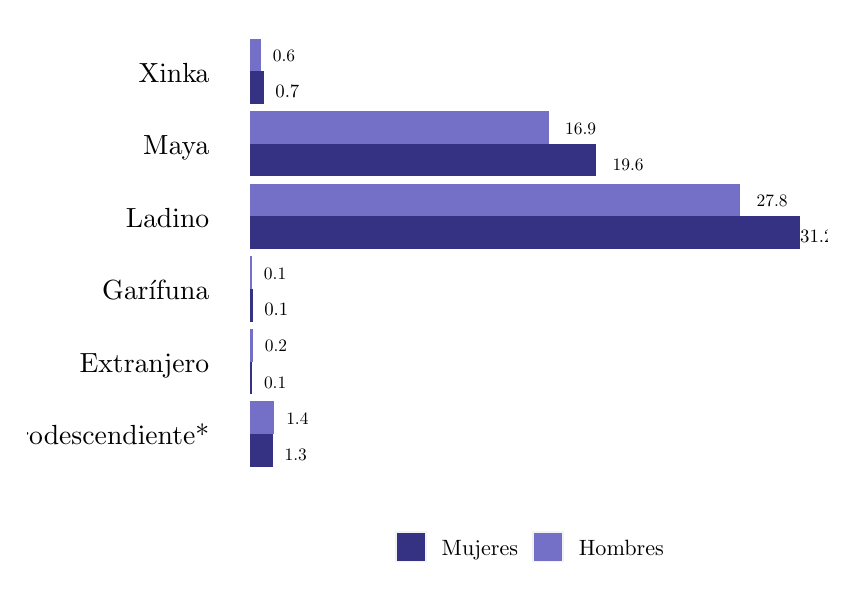
\begin{tikzpicture}[x=1pt,y=1pt]% Created by tikzDevice version 0.12.4 on 2023-05-02 12:30:50
% !TEX encoding = UTF-8 Unicode
\definecolor{fillColor}{RGB}{255,255,255}
\path[use as bounding box,fill=fillColor,fill opacity=0.00] (0,0) rectangle (289.08,198.74);
\begin{scope}
\path[clip] (  0.00,  0.00) rectangle (289.08,198.74);

\path[] (  0.00,  0.00) rectangle (289.08,198.74);
\end{scope}
\begin{scope}
\path[clip] (  0.00,  0.00) rectangle (289.08,198.74);
\definecolor{fillColor}{RGB}{54,50,131}

\path[fill=fillColor] ( 80.50,171.20) rectangle ( 85.23,183.01);

\path[fill=fillColor] ( 80.50, 92.52) rectangle ( 81.24,104.32);

\path[fill=fillColor] ( 80.50,118.75) rectangle (279.15,130.55);

\path[fill=fillColor] ( 80.50, 40.07) rectangle ( 88.59, 51.87);

\path[fill=fillColor] ( 80.50, 66.29) rectangle ( 81.13, 78.10);

\path[fill=fillColor] ( 80.50,144.98) rectangle (205.38,156.78);
\definecolor{fillColor}{RGB}{116,112,200}

\path[fill=fillColor] ( 80.50,183.01) rectangle ( 84.35,194.81);

\path[fill=fillColor] ( 80.50,104.32) rectangle ( 81.11,116.13);

\path[fill=fillColor] ( 80.50,130.55) rectangle (257.44,142.35);

\path[fill=fillColor] ( 80.50, 51.87) rectangle ( 89.16, 63.67);

\path[fill=fillColor] ( 80.50, 78.10) rectangle ( 81.45, 89.90);

\path[fill=fillColor] ( 80.50,156.78) rectangle (188.23,168.58);
\definecolor{drawColor}{RGB}{0,0,0}

\node[text=drawColor,anchor=base west,inner sep=0pt, outer sep=0pt, scale=  0.68] at ( 89.50,173.42) {0.7};

\node[text=drawColor,anchor=base west,inner sep=0pt, outer sep=0pt, scale=  0.68] at ( 85.51, 94.73) {0.1};

\node[text=drawColor,anchor=base west,inner sep=0pt, outer sep=0pt, scale=  0.68] at (279.12,120.96) {31.2};

\node[text=drawColor,anchor=base west,inner sep=0pt, outer sep=0pt, scale=  0.63] at ( 92.86, 42.28) {1.3};

\node[text=drawColor,anchor=base west,inner sep=0pt, outer sep=0pt, scale=  0.63] at ( 85.40, 68.51) {0.1};

\node[text=drawColor,anchor=base west,inner sep=0pt, outer sep=0pt, scale=  0.63] at (211.36,147.19) {19.6};

\node[text=drawColor,anchor=base west,inner sep=0pt, outer sep=0pt, scale=  0.63] at ( 88.62,186.53) {0.6};

\node[text=drawColor,anchor=base west,inner sep=0pt, outer sep=0pt, scale=  0.63] at ( 85.38,107.85) {0.1};

\node[text=drawColor,anchor=base west,inner sep=0pt, outer sep=0pt, scale=  0.63] at (263.41,134.07) {27.8};

\node[text=drawColor,anchor=base west,inner sep=0pt, outer sep=0pt, scale=  0.63] at ( 93.44, 55.39) {1.4};

\node[text=drawColor,anchor=base west,inner sep=0pt, outer sep=0pt, scale=  0.63] at ( 85.73, 81.62) {0.2};

\node[text=drawColor,anchor=base west,inner sep=0pt, outer sep=0pt, scale=  0.63] at (194.20,160.30) {16.9};

\path[] ( 70.56, 51.87) --
	(289.08, 51.87);

\path[] ( 70.56, 78.10) --
	(289.08, 78.10);

\path[] ( 70.56,104.32) --
	(289.08,104.32);

\path[] ( 70.56,130.55) --
	(289.08,130.55);

\path[] ( 70.56,156.78) --
	(289.08,156.78);

\path[] ( 70.56,183.01) --
	(289.08,183.01);

\path[] ( 70.56, 36.13) rectangle (289.08,198.74);
\end{scope}
\begin{scope}
\path[clip] (  0.00,  0.00) rectangle (289.08,198.74);

\path[] ( 70.56, 36.13) --
	( 70.56,198.74);
\end{scope}
\begin{scope}
\path[clip] (  0.00,  0.00) rectangle (289.08,198.74);
\definecolor{drawColor}{RGB}{0,0,0}

\node[text=drawColor,anchor=base east,inner sep=0pt, outer sep=0pt, scale=  1.00] at ( 65.61, 47.96) {Afrodescendiente*};

\node[text=drawColor,anchor=base east,inner sep=0pt, outer sep=0pt, scale=  1.00] at ( 65.61, 74.19) {Extranjero};

\node[text=drawColor,anchor=base east,inner sep=0pt, outer sep=0pt, scale=  1.00] at ( 65.61,100.41) {Garífuna};

\node[text=drawColor,anchor=base east,inner sep=0pt, outer sep=0pt, scale=  1.00] at ( 65.61,126.64) {Ladino};

\node[text=drawColor,anchor=base east,inner sep=0pt, outer sep=0pt, scale=  1.00] at ( 65.61,152.87) {Maya};

\node[text=drawColor,anchor=base east,inner sep=0pt, outer sep=0pt, scale=  1.00] at ( 65.61,179.10) {Xinka};
\end{scope}
\begin{scope}
\path[clip] (  0.00,  0.00) rectangle (289.08,198.74);

\path[] ( 67.81, 51.87) --
	( 70.56, 51.87);

\path[] ( 67.81, 78.10) --
	( 70.56, 78.10);

\path[] ( 67.81,104.32) --
	( 70.56,104.32);

\path[] ( 67.81,130.55) --
	( 70.56,130.55);

\path[] ( 67.81,156.78) --
	( 70.56,156.78);

\path[] ( 67.81,183.01) --
	( 70.56,183.01);
\end{scope}
\begin{scope}
\path[clip] (  0.00,  0.00) rectangle (289.08,198.74);

\path[] ( 70.56, 36.13) --
	(289.08, 36.13);
\end{scope}
\begin{scope}
\path[clip] (  0.00,  0.00) rectangle (289.08,198.74);

\path[] ( 80.50, 33.38) --
	( 80.50, 36.13);

\path[] (144.15, 33.38) --
	(144.15, 36.13);

\path[] (207.80, 33.38) --
	(207.80, 36.13);

\path[] (271.45, 33.38) --
	(271.45, 36.13);
\end{scope}
\begin{scope}
\path[clip] (  0.00,  0.00) rectangle (289.08,198.74);
\definecolor{fillColor}{RGB}{255,255,255}

\path[fill=fillColor] (131.74, -0.00) rectangle (227.91, 22.38);
\end{scope}
\begin{scope}
\path[clip] (  0.00,  0.00) rectangle (289.08,198.74);
\definecolor{fillColor}{gray}{0.95}

\path[fill=fillColor] (132.74,  5.50) rectangle (144.12, 16.88);
\end{scope}
\begin{scope}
\path[clip] (  0.00,  0.00) rectangle (289.08,198.74);
\definecolor{fillColor}{RGB}{54,50,131}

\path[fill=fillColor] (133.40,  6.16) rectangle (143.46, 16.22);  %cuadro leyenda mujeres
\end{scope}
\begin{scope}
\path[clip] (  0.00,  0.00) rectangle (289.08,198.74);
\definecolor{fillColor}{gray}{0.95}

\path[fill=fillColor] (182.28,  5.50) rectangle (193.66, 16.88);
\end{scope}
\begin{scope}
\path[clip] (  0.00,  0.00) rectangle (289.08,198.74);
\definecolor{fillColor}{RGB}{116,112,200}

\path[fill=fillColor] (182.94,  6.16) rectangle (193.00, 16.22);
\end{scope}
\begin{scope}
\path[clip] (  0.00,  0.00) rectangle (289.08,198.74);
\definecolor{drawColor}{RGB}{0,0,0}

\node[text=drawColor,anchor=base west,inner sep=0pt, outer sep=0pt, scale=  0.80] at (149.62,  8.06) {Mujeres};
\end{scope}
\begin{scope}
\path[clip] (  0.00,  0.00) rectangle (289.08,198.74);
\definecolor{drawColor}{RGB}{0,0,0}

\node[text=drawColor,anchor=base west,inner sep=0pt, outer sep=0pt, scale=  0.80] at (199.16,  8.06) {Hombres};
\end{scope}
\end{tikzpicture}}{INE - ENEI 2022}{}

\cajota{Población por sexo, según comunidad lingüística}{Para el 2018, se muestra el número de personas por sexo pertenecientes a las 22 comunidades lingüísticas Maya. Se observa que en la mayoría de comunidades existe una mayor población de mujeres, con excepción de la comunidad Itza’.}{Población por sexo, según comunidad lingüística}{República de Guatemala, Instituto Nacional de Estadística -INE-, en número de personas}{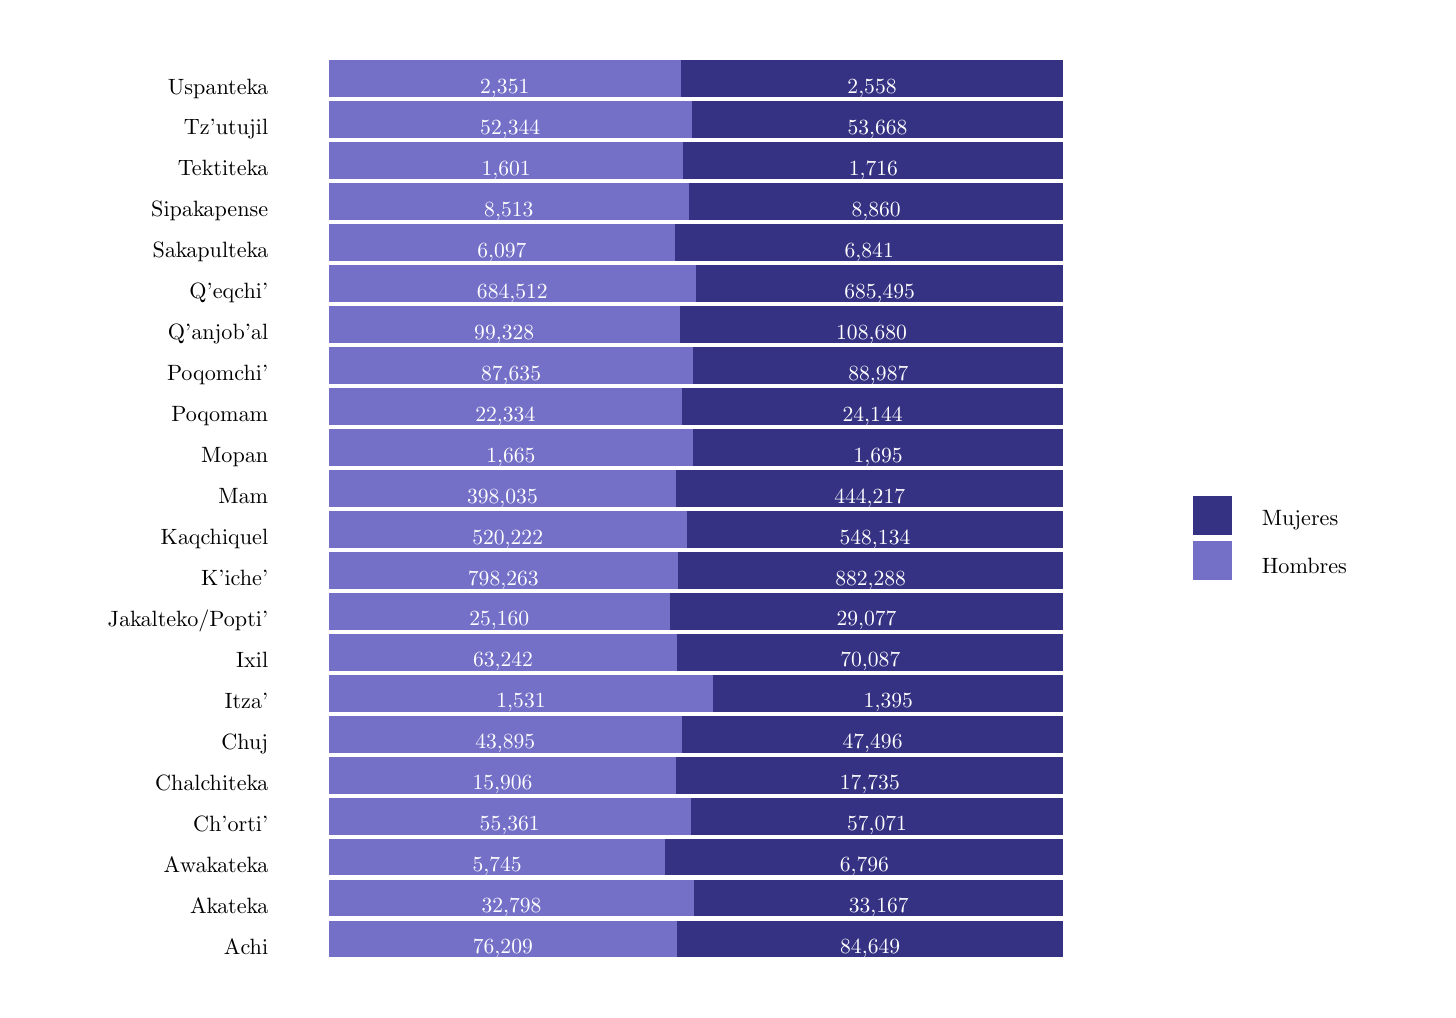
\begin{tikzpicture}[x=1pt,y=1pt, , scale=1.75]% Created by tikzDevice version 0.12.4 on 2023-05-08 10:54:28
% !TEX encoding = UTF-8 Unicode
\definecolor{fillColor}{RGB}{255,255,255}
\path[use as bounding box,fill=fillColor,fill opacity=0.00] (0,0) rectangle (289.08,198.74);
\begin{scope}
\path[clip] (  0.00,  0.00) rectangle (289.08,198.74);
\definecolor{drawColor}{RGB}{255,255,255}
\definecolor{fillColor}{RGB}{255,255,255}

\path[draw=drawColor,line width= 0.6pt,line join=round,line cap=round,fill=fillColor] (  0.00,  0.00) rectangle (289.08,198.74);
\end{scope}
\begin{scope}
\path[clip] (  0.00,  0.00) rectangle (289.08,198.74);
\definecolor{fillColor}{RGB}{54,50,131}

\path[fill=fillColor] (134.05,  6.77) rectangle (213.87, 14.38);

\path[fill=fillColor] (137.61, 15.23) rectangle (213.87, 22.84);

\path[fill=fillColor] (131.67, 23.68) rectangle (213.87, 31.29);

\path[fill=fillColor] (136.88, 32.14) rectangle (213.87, 39.75);

\path[fill=fillColor] (133.91, 40.60) rectangle (213.87, 48.21);

\path[fill=fillColor] (135.04, 49.05) rectangle (213.87, 56.66);

\path[fill=fillColor] (141.56, 57.51) rectangle (213.87, 65.12);

\path[fill=fillColor] (134.14, 65.97) rectangle (213.87, 73.58);

\path[fill=fillColor] (132.55, 74.42) rectangle (213.87, 82.03);

\path[fill=fillColor] (134.24, 82.88) rectangle (213.87, 90.49);

\path[fill=fillColor] (136.05, 91.34) rectangle (213.87, 98.95);

\path[fill=fillColor] (133.87, 99.79) rectangle (213.87,107.41);

\path[fill=fillColor] (137.35,108.25) rectangle (213.87,115.86);

\path[fill=fillColor] (135.08,116.71) rectangle (213.87,124.32);

\path[fill=fillColor] (137.45,125.16) rectangle (213.87,132.78);

\path[fill=fillColor] (134.62,133.62) rectangle (213.87,141.23);

\path[fill=fillColor] (137.98,142.08) rectangle (213.87,149.69);

\path[fill=fillColor] (133.67,150.54) rectangle (213.87,158.15);

\path[fill=fillColor] (136.52,158.99) rectangle (213.87,166.60);

\path[fill=fillColor] (135.40,167.45) rectangle (213.87,175.06);

\path[fill=fillColor] (137.08,175.91) rectangle (213.87,183.52);

\path[fill=fillColor] (134.83,184.36) rectangle (213.87,191.97);
\definecolor{fillColor}{RGB}{116,112,200}

\path[fill=fillColor] ( 62.19,  6.77) rectangle (134.05, 14.38);

\path[fill=fillColor] ( 62.19, 15.23) rectangle (137.61, 22.84);

\path[fill=fillColor] ( 62.19, 23.68) rectangle (131.67, 31.29);

\path[fill=fillColor] ( 62.19, 32.14) rectangle (136.88, 39.75);

\path[fill=fillColor] ( 62.19, 40.60) rectangle (133.91, 48.21);

\path[fill=fillColor] ( 62.19, 49.05) rectangle (135.04, 56.66);

\path[fill=fillColor] ( 62.19, 57.51) rectangle (141.56, 65.12);

\path[fill=fillColor] ( 62.19, 65.97) rectangle (134.14, 73.58);

\path[fill=fillColor] ( 62.19, 74.42) rectangle (132.55, 82.03);

\path[fill=fillColor] ( 62.19, 82.88) rectangle (134.24, 90.49);

\path[fill=fillColor] ( 62.19, 91.34) rectangle (136.05, 98.95);

\path[fill=fillColor] ( 62.19, 99.79) rectangle (133.87,107.41);

\path[fill=fillColor] ( 62.19,108.25) rectangle (137.35,115.86);

\path[fill=fillColor] ( 62.19,116.71) rectangle (135.08,124.32);

\path[fill=fillColor] ( 62.19,125.16) rectangle (137.45,132.78);

\path[fill=fillColor] ( 62.19,133.62) rectangle (134.62,141.23);

\path[fill=fillColor] ( 62.19,142.08) rectangle (137.98,149.69);

\path[fill=fillColor] ( 62.19,150.54) rectangle (133.67,158.15);

\path[fill=fillColor] ( 62.19,158.99) rectangle (136.52,166.60);

\path[fill=fillColor] ( 62.19,167.45) rectangle (135.40,175.06);

\path[fill=fillColor] ( 62.19,175.91) rectangle (137.08,183.52);

\path[fill=fillColor] ( 62.19,184.36) rectangle (134.83,191.97);
\definecolor{drawColor}{RGB}{255,255,255}

\node[text=drawColor,anchor=base,inner sep=0pt, outer sep=0pt, scale=  0.78] at (173.96,  7.54) {84,649};

\node[text=drawColor,anchor=base,inner sep=0pt, outer sep=0pt, scale=  0.78] at (175.74, 16.00) {33,167};

\node[text=drawColor,anchor=base,inner sep=0pt, outer sep=0pt, scale=  0.78] at (172.77, 24.45) {6,796};

\node[text=drawColor,anchor=base,inner sep=0pt, outer sep=0pt, scale=  0.78] at (175.37, 32.91) {57,071};

\node[text=drawColor,anchor=base,inner sep=0pt, outer sep=0pt, scale=  0.78] at (173.89, 41.37) {17,735};

\node[text=drawColor,anchor=base,inner sep=0pt, outer sep=0pt, scale=  0.78] at (174.46, 49.83) {47,496};

\node[text=drawColor,anchor=base,inner sep=0pt, outer sep=0pt, scale=  0.78] at (177.71, 58.28) {1,395};

\node[text=drawColor,anchor=base,inner sep=0pt, outer sep=0pt, scale=  0.78] at (174.00, 66.74) {70,087};

\node[text=drawColor,anchor=base,inner sep=0pt, outer sep=0pt, scale=  0.78] at (173.21, 75.20) {29,077};

\node[text=drawColor,anchor=base,inner sep=0pt, outer sep=0pt, scale=  0.78] at (174.06, 83.65) {882,288};

\node[text=drawColor,anchor=base,inner sep=0pt, outer sep=0pt, scale=  0.78] at (174.96, 92.11) {548,134};

\node[text=drawColor,anchor=base,inner sep=0pt, outer sep=0pt, scale=  0.78] at (173.87,100.57) {444,217};

\node[text=drawColor,anchor=base,inner sep=0pt, outer sep=0pt, scale=  0.78] at (175.61,109.02) {1,695};

\node[text=drawColor,anchor=base,inner sep=0pt, outer sep=0pt, scale=  0.78] at (174.47,117.48) {24,144};

\node[text=drawColor,anchor=base,inner sep=0pt, outer sep=0pt, scale=  0.78] at (175.66,125.94) {88,987};

\node[text=drawColor,anchor=base,inner sep=0pt, outer sep=0pt, scale=  0.78] at (174.25,134.39) {108,680};

\node[text=drawColor,anchor=base,inner sep=0pt, outer sep=0pt, scale=  0.78] at (175.92,142.85) {685,495};

\node[text=drawColor,anchor=base,inner sep=0pt, outer sep=0pt, scale=  0.78] at (173.77,151.31) {6,841};

\node[text=drawColor,anchor=base,inner sep=0pt, outer sep=0pt, scale=  0.78] at (175.19,159.76) {8,860};

\node[text=drawColor,anchor=base,inner sep=0pt, outer sep=0pt, scale=  0.78] at (174.64,168.22) {1,716};

\node[text=drawColor,anchor=base,inner sep=0pt, outer sep=0pt, scale=  0.78] at (175.48,176.68) {53,668};

\node[text=drawColor,anchor=base,inner sep=0pt, outer sep=0pt, scale=  0.78] at (174.35,185.14) {2,558};

\node[text=drawColor,anchor=base,inner sep=0pt, outer sep=0pt, scale=  0.78] at ( 98.12,  7.54) {76,209};

\node[text=drawColor,anchor=base,inner sep=0pt, outer sep=0pt, scale=  0.78] at ( 99.90, 16.00) {32,798};

\node[text=drawColor,anchor=base,inner sep=0pt, outer sep=0pt, scale=  0.78] at ( 96.93, 24.45) {5,745};

\node[text=drawColor,anchor=base,inner sep=0pt, outer sep=0pt, scale=  0.78] at ( 99.53, 32.91) {55,361};

\node[text=drawColor,anchor=base,inner sep=0pt, outer sep=0pt, scale=  0.78] at ( 98.05, 41.37) {15,906};

\node[text=drawColor,anchor=base,inner sep=0pt, outer sep=0pt, scale=  0.78] at ( 98.62, 49.83) {43,895};

\node[text=drawColor,anchor=base,inner sep=0pt, outer sep=0pt, scale=  0.78] at (101.87, 58.28) {1,531};

\node[text=drawColor,anchor=base,inner sep=0pt, outer sep=0pt, scale=  0.78] at ( 98.16, 66.74) {63,242};

\node[text=drawColor,anchor=base,inner sep=0pt, outer sep=0pt, scale=  0.78] at ( 97.37, 75.20) {25,160};

\node[text=drawColor,anchor=base,inner sep=0pt, outer sep=0pt, scale=  0.78] at ( 98.21, 83.65) {798,263};

\node[text=drawColor,anchor=base,inner sep=0pt, outer sep=0pt, scale=  0.78] at ( 99.12, 92.11) {520,222};

\node[text=drawColor,anchor=base,inner sep=0pt, outer sep=0pt, scale=  0.78] at ( 98.03,100.57) {398,035};

\node[text=drawColor,anchor=base,inner sep=0pt, outer sep=0pt, scale=  0.78] at ( 99.77,109.02) {1,665};

\node[text=drawColor,anchor=base,inner sep=0pt, outer sep=0pt, scale=  0.78] at ( 98.63,117.48) {22,334};

\node[text=drawColor,anchor=base,inner sep=0pt, outer sep=0pt, scale=  0.78] at ( 99.82,125.94) {87,635};

\node[text=drawColor,anchor=base,inner sep=0pt, outer sep=0pt, scale=  0.78] at ( 98.40,134.39) {99,328};

\node[text=drawColor,anchor=base,inner sep=0pt, outer sep=0pt, scale=  0.78] at (100.08,142.85) {684,512};

\node[text=drawColor,anchor=base,inner sep=0pt, outer sep=0pt, scale=  0.78] at ( 97.93,151.31) {6,097};

\node[text=drawColor,anchor=base,inner sep=0pt, outer sep=0pt, scale=  0.78] at ( 99.35,159.76) {8,513};

\node[text=drawColor,anchor=base,inner sep=0pt, outer sep=0pt, scale=  0.78] at ( 98.80,168.22) {1,601};

\node[text=drawColor,anchor=base,inner sep=0pt, outer sep=0pt, scale=  0.78] at ( 99.64,176.68) {52,344};

\node[text=drawColor,anchor=base,inner sep=0pt, outer sep=0pt, scale=  0.78] at ( 98.51,185.14) {2,351};
\end{scope}
\begin{scope}
\path[clip] (  0.00,  0.00) rectangle (289.08,198.74);
\definecolor{drawColor}{RGB}{0,0,0}

\node[text=drawColor,anchor=base east,inner sep=0pt, outer sep=0pt, scale=  0.80] at ( 49.66,  7.45) {Achi};

\node[text=drawColor,anchor=base east,inner sep=0pt, outer sep=0pt, scale=  0.80] at ( 49.66, 15.90) {Akateka};

\node[text=drawColor,anchor=base east,inner sep=0pt, outer sep=0pt, scale=  0.80] at ( 49.66, 24.36) {Awakateka};

\node[text=drawColor,anchor=base east,inner sep=0pt, outer sep=0pt, scale=  0.80] at ( 49.66, 32.82) {Ch'orti'};

\node[text=drawColor,anchor=base east,inner sep=0pt, outer sep=0pt, scale=  0.80] at ( 49.66, 41.27) {Chalchiteka};

\node[text=drawColor,anchor=base east,inner sep=0pt, outer sep=0pt, scale=  0.80] at ( 49.66, 49.73) {Chuj};

\node[text=drawColor,anchor=base east,inner sep=0pt, outer sep=0pt, scale=  0.80] at ( 49.66, 58.19) {Itza'};

\node[text=drawColor,anchor=base east,inner sep=0pt, outer sep=0pt, scale=  0.80] at ( 49.66, 66.65) {Ixil};

\node[text=drawColor,anchor=base east,inner sep=0pt, outer sep=0pt, scale=  0.80] at ( 49.66, 75.10) {Jakalteko/Popti'};

\node[text=drawColor,anchor=base east,inner sep=0pt, outer sep=0pt, scale=  0.80] at ( 49.66, 83.56) {K'iche'};

\node[text=drawColor,anchor=base east,inner sep=0pt, outer sep=0pt, scale=  0.80] at ( 49.66, 92.02) {Kaqchiquel};

\node[text=drawColor,anchor=base east,inner sep=0pt, outer sep=0pt, scale=  0.80] at ( 49.66,100.47) {Mam};

\node[text=drawColor,anchor=base east,inner sep=0pt, outer sep=0pt, scale=  0.80] at ( 49.66,108.93) {Mopan};

\node[text=drawColor,anchor=base east,inner sep=0pt, outer sep=0pt, scale=  0.80] at ( 49.66,117.39) {Poqomam};

\node[text=drawColor,anchor=base east,inner sep=0pt, outer sep=0pt, scale=  0.80] at ( 49.66,125.84) {Poqomchi'};

\node[text=drawColor,anchor=base east,inner sep=0pt, outer sep=0pt, scale=  0.80] at ( 49.66,134.30) {Q'anjob'al};

\node[text=drawColor,anchor=base east,inner sep=0pt, outer sep=0pt, scale=  0.80] at ( 49.66,142.76) {Q'eqchi'};

\node[text=drawColor,anchor=base east,inner sep=0pt, outer sep=0pt, scale=  0.80] at ( 49.66,151.21) {Sakapulteka};

\node[text=drawColor,anchor=base east,inner sep=0pt, outer sep=0pt, scale=  0.80] at ( 49.66,159.67) {Sipakapense};

\node[text=drawColor,anchor=base east,inner sep=0pt, outer sep=0pt, scale=  0.80] at ( 49.66,168.13) {Tektiteka};

\node[text=drawColor,anchor=base east,inner sep=0pt, outer sep=0pt, scale=  0.80] at ( 49.66,176.58) {Tz'utujil};

\node[text=drawColor,anchor=base east,inner sep=0pt, outer sep=0pt, scale=  0.80] at ( 49.66,185.04) {Uspanteka};
\end{scope}
\begin{scope}
\path[clip] (  0.00,  0.00) rectangle (289.08,198.74);
\definecolor{fillColor}{RGB}{255,255,255}

\path[fill=fillColor] (232.46, 74.52) rectangle (283.58,124.23);
\end{scope}
\begin{scope}
\path[clip] (  0.00,  0.00) rectangle (289.08,198.74);
\definecolor{fillColor}{gray}{0.95}

%\path[fill=fillColor] (237.96, 91.40) rectangle (249.34,102.78);
\end{scope}
\begin{scope}
\path[clip] (  0.00,  0.00) rectangle (289.08,198.74);
\definecolor{fillColor}{RGB}{54,50,131}

\path[fill=fillColor] (240.62, 94.06) rectangle (248.67,102.12);
\end{scope}
\begin{scope}
\path[clip] (  0.00,  0.00) rectangle (289.08,198.74);
\definecolor{fillColor}{gray}{0.95}

%\path[fill=fillColor] (237.96, 80.02) rectangle (249.34, 91.40);
\end{scope}
\begin{scope}
\path[clip] (  0.00,  0.00) rectangle (289.08,198.74);
\definecolor{fillColor}{RGB}{116,112,200}

\path[fill=fillColor] (240.62, 84.68) rectangle (248.67, 92.74);
\end{scope}
\begin{scope}
\path[clip] (  0.00,  0.00) rectangle (289.08,198.74);
\definecolor{drawColor}{RGB}{0,0,0}

\node[text=drawColor,anchor=base west,inner sep=0pt, outer sep=0pt, scale=  0.80] at (254.84, 95.96) {Mujeres};
\end{scope}
\begin{scope}
\path[clip] (  0.00,  0.00) rectangle (289.08,198.74);
\definecolor{drawColor}{RGB}{0,0,0}

\node[text=drawColor,anchor=base west,inner sep=0pt, outer sep=0pt, scale=  0.80] at (254.84, 85.98) {Hombres};
\end{scope}
\end{tikzpicture}}{INE - Censo 2018}

%\cajita{Población por sexo, según tipo de hogar (PENDIENTE)}{Los tipos de hogar son clasificados de la siguiente forma:}{Población por sexo, según tipo de hogar}{República de Guatemala, Instituto Nacional de Estadística -INE-, en porcentaje}{\begin{tikzpicture}[x=1pt,y=1pt]% Created by tikzDevice version 0.12.4 on 2023-04-20 12:31:17
% !TEX encoding = UTF-8 Unicode
\end{tikzpicture}}{INE - ENEI 2022}{}

%\cajita{Población por sexo, según tipo de vivienda (PENDIENTE)}{Los tipos de hogar son clasificados de la siguiente forma:}{Población por sexo, según tipo de hogar}{República de Guatemala, Instituto Nacional de Estadística -INE-, en porcentaje}{\begin{tikzpicture}[x=1pt,y=1pt]% Created by tikzDevice version 0.12.4 on 2023-04-20 12:31:17
% !TEX encoding = UTF-8 Unicode
\end{tikzpicture}}{INE - ENEI 2022}{}

\cajota{Mapa departamental por número de mujeres}{Este es un mapa departamental por sexo :)}{Proyección de población de mujeres por departamento}{República de Guatemala, Instituto Nacional de Estadística -INE-, en número de mujeres}{\includegraphics[width=0.75\textwidth]{Graficas/mapa_departamental}}{INE - Proyecciones 2020}

\cajota{Mapa municipal por número de mujeres}{Para 2022, según estimaciones del Instituto Nacional de Estadística, el municipio con mayor población de mujeres fue el municipio de Guatemala con 630,634 mujeres, seguido de Mixco con 269,358 mujeres. Los municipios con menor proyección poblacional de mujeres fueron Santa María Visitación con 1,354 mujeres y San Marcos La Laguna con 1,531 mujeres.  }{Proyección de población de mujeres por municipio}{República de Guatemala, Instituto Nacional de Estadística -INE-, en número de mujeres}{\includegraphics[width=0.75\textwidth]{Graficas/mapa_municipal}}{INE - Proyecciones 2020}

\cajita{Esperanza de vida al nacer por sexo}{La esperanza de vida al nacer indica la cantidad de años que se espera que viva la persona nacida en un periodo de tiempo determinado. En Guatemala, las mujeres tienen una esperanza de vida mayor que los hombres. El período de referencia es tomado hasta el 30 junio de cada año. }{Serie histórica de esperanza de vida}{República de Guatemala, Instituto Nacional de Estadística -INE-, en número de años}{\begin{tikzpicture}[x=1pt,y=1pt]% Created by tikzDevice version 0.12.4 on 2023-05-15 10:48:14
% !TEX encoding = UTF-8 Unicode
\definecolor{fillColor}{RGB}{255,255,255}
\path[use as bounding box,fill=fillColor,fill opacity=0.00] (0,0) rectangle (289.08,198.74);
\begin{scope}
\path[clip] (  0.00,  0.00) rectangle (289.08,198.74);

\path[] (  0.00,  0.00) rectangle (289.08,198.74);
\end{scope}
\begin{scope}
\path[clip] (  0.00,  0.00) rectangle (289.08,198.74);
\definecolor{drawColor}{RGB}{54,50,131}

\path[draw=drawColor,line width= 1.7pt,line join=round] ( 31.91,128.88) --
	( 85.96,130.22) --
	(140.01,131.55) --
	(194.06,132.89) --
	(248.11,134.22);
\definecolor{drawColor}{RGB}{116,112,200}

\path[draw=drawColor,line width= 1.7pt,line join=round] ( 31.91, 85.49) --
	( 85.96, 86.82) --
	(140.01, 88.16) --
	(194.06, 89.49) --
	(248.11, 90.83);
\definecolor{drawColor}{RGB}{0,0,0}

\node[text=drawColor,anchor=base,inner sep=0pt, outer sep=0pt, scale=  1.02] at ( 31.91,116.97) {75.8};

\node[text=drawColor,anchor=base east,inner sep=0pt, outer sep=0pt, scale=  1.02] at ( 82.83,130.22) {76.0};

\node[text=drawColor,anchor=base east,inner sep=0pt, outer sep=0pt, scale=  1.02] at (136.88,131.55) {76.2};

\node[text=drawColor,anchor=base east,inner sep=0pt, outer sep=0pt, scale=  1.02] at (190.94,132.89) {76.4};

\node[text=drawColor,anchor=base,inner sep=0pt, outer sep=0pt, scale=  1.02] at (248.11,138.19) {76.6};

\node[text=drawColor,anchor=base,inner sep=0pt, outer sep=0pt, scale=  1.02] at ( 31.91, 73.58) {69.3};

\node[text=drawColor,anchor=base east,inner sep=0pt, outer sep=0pt, scale=  1.02] at ( 82.83, 86.82) {69.5};

\node[text=drawColor,anchor=base east,inner sep=0pt, outer sep=0pt, scale=  1.02] at (136.88, 88.16) {69.7};

\node[text=drawColor,anchor=base east,inner sep=0pt, outer sep=0pt, scale=  1.02] at (190.94, 89.49) {69.9};

\node[text=drawColor,anchor=base,inner sep=0pt, outer sep=0pt, scale=  1.02] at (248.11, 94.80) {70.1};

\path[draw=drawColor,line width= 0.1pt,line join=round] (-281.58, 23.41) -- (561.61, 23.41);

\path[] ( -0.52, 15.40) rectangle (280.54,191.63);

\path[] ( -0.52, 40.10) --
	(280.54, 40.10);

\path[] ( -0.52, 73.47) --
	(280.54, 73.47);

\path[] ( -0.52,106.85) --
	(280.54,106.85);

\path[] ( -0.52,140.23) --
	(280.54,140.23);

\path[] ( -0.52,173.61) --
	(280.54,173.61);

\path[] ( -0.52, 23.41) --
	(280.54, 23.41);

\path[] ( -0.52, 56.79) --
	(280.54, 56.79);

\path[] ( -0.52, 90.16) --
	(280.54, 90.16);

\path[] ( -0.52,123.54) --
	(280.54,123.54);

\path[] ( -0.52,156.92) --
	(280.54,156.92);

\path[] ( -0.52,190.29) --
	(280.54,190.29);

\path[] ( 31.91, 15.40) --
	( 31.91,191.63);

\path[] ( 85.96, 15.40) --
	( 85.96,191.63);

\path[] (140.01, 15.40) --
	(140.01,191.63);

\path[] (194.06, 15.40) --
	(194.06,191.63);

\path[] (248.11, 15.40) --
	(248.11,191.63);

\path[] ( -0.52, 15.40) rectangle (280.54,191.63);
\end{scope}
\begin{scope}
\path[clip] (  0.00,  0.00) rectangle (289.08,198.74);

\path[] ( -0.52, 15.40) --
	( -0.52,191.63);
\end{scope}
\begin{scope}
\path[clip] (  0.00,  0.00) rectangle (289.08,198.74);
\definecolor{drawColor}{RGB}{255,255,255}

\node[text=drawColor,text opacity=0.00,anchor=base east,inner sep=0pt, outer sep=0pt, scale=  1.00] at ( -5.47, 19.50) {60};

\node[text=drawColor,text opacity=0.00,anchor=base east,inner sep=0pt, outer sep=0pt, scale=  1.00] at ( -5.47, 52.88) {65};

\node[text=drawColor,text opacity=0.00,anchor=base east,inner sep=0pt, outer sep=0pt, scale=  1.00] at ( -5.47, 86.25) {70};

\node[text=drawColor,text opacity=0.00,anchor=base east,inner sep=0pt, outer sep=0pt, scale=  1.00] at ( -5.47,119.63) {75};

\node[text=drawColor,text opacity=0.00,anchor=base east,inner sep=0pt, outer sep=0pt, scale=  1.00] at ( -5.47,153.01) {80};

\node[text=drawColor,text opacity=0.00,anchor=base east,inner sep=0pt, outer sep=0pt, scale=  1.00] at ( -5.47,186.39) {85};
\end{scope}
\begin{scope}
\path[clip] (  0.00,  0.00) rectangle (289.08,198.74);

\path[] ( -3.27, 23.41) --
	( -0.52, 23.41);

\path[] ( -3.27, 56.79) --
	( -0.52, 56.79);

\path[] ( -3.27, 90.16) --
	( -0.52, 90.16);

\path[] ( -3.27,123.54) --
	( -0.52,123.54);

\path[] ( -3.27,156.92) --
	( -0.52,156.92);

\path[] ( -3.27,190.29) --
	( -0.52,190.29);
\end{scope}
\begin{scope}
\path[clip] (  0.00,  0.00) rectangle (289.08,198.74);

\path[] ( -0.52, 15.40) --
	(280.54, 15.40);
\end{scope}
\begin{scope}
\path[clip] (  0.00,  0.00) rectangle (289.08,198.74);

\path[] ( 31.91, 12.65) --
	( 31.91, 15.40);

\path[] ( 85.96, 12.65) --
	( 85.96, 15.40);

\path[] (140.01, 12.65) --
	(140.01, 15.40);

\path[] (194.06, 12.65) --
	(194.06, 15.40);

\path[] (248.11, 12.65) --
	(248.11, 15.40);
\end{scope}
\begin{scope}
\path[clip] (  0.00,  0.00) rectangle (289.08,198.74);
\definecolor{drawColor}{RGB}{0,0,0}

\node[text=drawColor,anchor=base,inner sep=0pt, outer sep=0pt, scale=  1.00] at ( 31.91,  1.32) {2017-2018};

\node[text=drawColor,anchor=base,inner sep=0pt, outer sep=0pt, scale=  1.00] at ( 85.96,  1.32) {2018-2019};

\node[text=drawColor,anchor=base,inner sep=0pt, outer sep=0pt, scale=  1.00] at (140.01,  1.32) {2019-2020};

\node[text=drawColor,anchor=base,inner sep=0pt, outer sep=0pt, scale=  1.00] at (194.06,  1.32) {2020-2021};

\node[text=drawColor,anchor=base,inner sep=0pt, outer sep=0pt, scale=  1.00] at (248.11,  1.32) {2021-2022};
\end{scope}
\begin{scope}
\path[clip] (  0.00,  0.00) rectangle (289.08,198.74);
\coordinate (apoyo) at (54.45,189.21);
\coordinate (longitudFicticia) at (7.11,9.53);
\coordinate (longitud) at (7.11,7.11);
\coordinate (desX) at (137.12,0);
\coordinate (desY) at (0,1.21);
\definecolor[named]{ct1}{HTML}{
363283
}
\definecolor[named]{ct2}{HTML}{
7470C8
}
\definecolor[named]{ctb1}{HTML}{
363283
}
\definecolor[named]{ctb2}{HTML}{
7470C8
}
\path [fill=none] (apoyo) rectangle ($(apoyo)+(longitudFicticia)$)
node [xshift=0.3cm,inner sep=0pt, outer sep=0pt,midway,right,scale = 1]{Mujeres};
\draw [color = ctb1,fill=ct1] ( $(apoyo)  + (desY) $) rectangle ($(apoyo)+ (desY) +(longitud)$);
\path [fill=none] ($(apoyo)+(desX)$) rectangle ($(apoyo)+(desX)+(longitudFicticia)$)
node [xshift=0.3cm,inner sep=0pt, outer sep=0pt,midway,right,scale = 1]{Hombres};
\draw [color = ctb2 ,fill=ct2] ( $(apoyo)  + (desY) + (desX) $) rectangle ($(apoyo)+ (desY)+ (desX) +(longitud)$);
\end{scope}
\end{tikzpicture}}{INE y CELADE - 2019}{}

\cajita{Tasa global de fecundidad (mujeres 15 a 49 años)}{El valor de la Tasa Global de Fecundidad (TGF) se interpreta como el número de hijos e hijas, que en promedio tendría una mujer de una cohorte hipotética de mujeres no expuestas al riesgo de muerte desde el inicio hasta el fin del periodo fértil y que, a partir del momento en que se inicia la reproducción están expuestas a las tasas de fecundidad por edad de la población en estudio. 

En Guatemala tanto en 2020 como en 2021 se reportó la misma tasa de 2.3 hijas(os) por mujer.}{Serie histórica de tasa global de fecundidad}{República de Guatemala, Instituto Nacional de Estadística -INE-, en número de hijas(os)}{\begin{tikzpicture}[x=1pt,y=1pt]% Created by tikzDevice version 0.12.4 on 2023-04-21 15:59:15
% !TEX encoding = UTF-8 Unicode
\definecolor{fillColor}{RGB}{255,255,255}
\path[use as bounding box,fill=fillColor,fill opacity=0.00] (0,0) rectangle (289.08,198.74);
\begin{scope}
\path[clip] (  0.00,  0.00) rectangle (289.08,198.74);

\path[] (  0.00,  0.00) rectangle (289.08,198.74);
\end{scope}
\begin{scope}
\path[clip] (  0.00,  0.00) rectangle (289.08,198.74);
\definecolor{drawColor}{RGB}{54,50,131}

\path[draw=drawColor,line width= 1.7pt,line join=round] ( 48.88, 67.15) --
	(113.23, 68.90) --
	(177.58,133.72) --
	(241.93,181.76);
\definecolor{drawColor}{RGB}{0,0,0}

\node[text=drawColor,anchor=base,inner sep=0pt, outer sep=0pt, scale=  1.02] at ( 48.88, 55.23) {2.3};

\node[text=drawColor,anchor=base east,inner sep=0pt, outer sep=0pt, scale=  1.02] at (111.00, 68.90) {2.3};

\node[text=drawColor,anchor=base east,inner sep=0pt, outer sep=0pt, scale=  1.02] at (175.35,133.72) {2.5};

\node[text=drawColor,anchor=base,inner sep=0pt, outer sep=0pt, scale=  1.02] at (241.93,185.73) {2.6};

\path[draw=drawColor,line width= 0.1pt,line join=round] (-260.00, 32.76) -- (550.81, 32.76);

\path[] ( 10.27, 25.31) rectangle (280.54,189.21);

\path[] ( 10.27, 33.20) --
	(280.54, 33.20);

\path[] ( 10.27, 64.32) --
	(280.54, 64.32);

\path[] ( 10.27, 95.43) --
	(280.54, 95.43);

\path[] ( 10.27,126.54) --
	(280.54,126.54);

\path[] ( 10.27,157.66) --
	(280.54,157.66);

\path[] ( 10.27,188.77) --
	(280.54,188.77);

\path[] ( 10.27, 48.76) --
	(280.54, 48.76);

\path[] ( 10.27, 79.87) --
	(280.54, 79.87);

\path[] ( 10.27,110.99) --
	(280.54,110.99);

\path[] ( 10.27,142.10) --
	(280.54,142.10);

\path[] ( 10.27,173.22) --
	(280.54,173.22);

\path[] ( 48.88, 25.31) --
	( 48.88,189.21);

\path[] (113.23, 25.31) --
	(113.23,189.21);

\path[] (177.58, 25.31) --
	(177.58,189.21);

\path[] (241.93, 25.31) --
	(241.93,189.21);

\path[] ( 10.27, 25.31) rectangle (280.54,189.21);
\end{scope}
\begin{scope}
\path[clip] (  0.00,  0.00) rectangle (289.08,198.74);

\path[] ( 10.27, 25.31) --
	( 10.27,189.21);
\end{scope}
\begin{scope}
\path[clip] (  0.00,  0.00) rectangle (289.08,198.74);
\definecolor{drawColor}{RGB}{255,255,255}

\node[text=drawColor,text opacity=0.00,anchor=base east,inner sep=0pt, outer sep=0pt, scale=  1.00] at (  5.32, 44.85) {2.2};

\node[text=drawColor,text opacity=0.00,anchor=base east,inner sep=0pt, outer sep=0pt, scale=  1.00] at (  5.32, 75.96) {2.3};

\node[text=drawColor,text opacity=0.00,anchor=base east,inner sep=0pt, outer sep=0pt, scale=  1.00] at (  5.32,107.08) {2.4};

\node[text=drawColor,text opacity=0.00,anchor=base east,inner sep=0pt, outer sep=0pt, scale=  1.00] at (  5.32,138.19) {2.5};

\node[text=drawColor,text opacity=0.00,anchor=base east,inner sep=0pt, outer sep=0pt, scale=  1.00] at (  5.32,169.31) {2.6};
\end{scope}
\begin{scope}
\path[clip] (  0.00,  0.00) rectangle (289.08,198.74);

\path[] (  7.52, 48.76) --
	( 10.27, 48.76);

\path[] (  7.52, 79.87) --
	( 10.27, 79.87);

\path[] (  7.52,110.99) --
	( 10.27,110.99);

\path[] (  7.52,142.10) --
	( 10.27,142.10);

\path[] (  7.52,173.22) --
	( 10.27,173.22);
\end{scope}
\begin{scope}
\path[clip] (  0.00,  0.00) rectangle (289.08,198.74);

\path[] ( 10.27, 25.31) --
	(280.54, 25.31);
\end{scope}
\begin{scope}
\path[clip] (  0.00,  0.00) rectangle (289.08,198.74);

\path[] ( 48.88, 22.56) --
	( 48.88, 25.31);

\path[] (113.23, 22.56) --
	(113.23, 25.31);

\path[] (177.58, 22.56) --
	(177.58, 25.31);

\path[] (241.93, 22.56) --
	(241.93, 25.31);
\end{scope}
\begin{scope}
\path[clip] (  0.00,  0.00) rectangle (289.08,198.74);
\definecolor{drawColor}{RGB}{0,0,0}

\node[text=drawColor,rotate= 90.00,anchor=base east,inner sep=0pt, outer sep=0pt, scale=  1.00] at ( 52.79, 20.36) {2021};

\node[text=drawColor,rotate= 90.00,anchor=base east,inner sep=0pt, outer sep=0pt, scale=  1.00] at (117.14, 20.36) {2020};

\node[text=drawColor,rotate= 90.00,anchor=base east,inner sep=0pt, outer sep=0pt, scale=  1.00] at (181.49, 20.36) {2019};

\node[text=drawColor,rotate= 90.00,anchor=base east,inner sep=0pt, outer sep=0pt, scale=  1.00] at (245.84, 20.36) {2018};
\end{scope}
\end{tikzpicture}}{INE - Estadísticas Vitales}{}

\cajita{Tasa de fecundidad juvenil según edades simples (13 -19 años)}{La tasa específica de fecundidad es el número de nacimientos por cada mil mujeres en la edad de 15 a 19. En Guatemala se reportó en 2021 una tasa específica de fecundidad de 51.4 hijas(os) por cada mil mujeres.}{Tasa de fecundidad juvenil según edades simples (13 -19 años)}{República de Guatemala, Instituto Nacional de Estadística -INE-, en número de hijas(os)}{\begin{tikzpicture}[x=1pt,y=1pt]% Created by tikzDevice version 0.12.4 on 2023-04-24 14:16:56
% !TEX encoding = UTF-8 Unicode
\definecolor{fillColor}{RGB}{255,255,255}
\path[use as bounding box,fill=fillColor,fill opacity=0.00] (0,0) rectangle (289.08,198.74);
\begin{scope}
\path[clip] (  0.00,  0.00) rectangle (289.08,198.74);

\path[] (  0.00,  0.00) rectangle (289.08,198.74);
\end{scope}
\begin{scope}
\path[clip] (  0.00,  0.00) rectangle (289.08,198.74);
\definecolor{drawColor}{RGB}{54,50,131}

\path[draw=drawColor,line width= 1.7pt,line join=round] ( 39.63,181.44) --
	(106.55,136.50) --
	(173.47, 61.88) --
	(240.39, 72.67);
\definecolor{drawColor}{RGB}{0,0,0}

\node[text=drawColor,anchor=base,inner sep=0pt, outer sep=0pt, scale=  1.02] at ( 39.63,185.41) {60.1};

\node[text=drawColor,anchor=base west,inner sep=0pt, outer sep=0pt, scale=  1.02] at (106.55,140.47) {56.5};

\node[text=drawColor,anchor=base,inner sep=0pt, outer sep=0pt, scale=  1.02] at (173.47, 49.97) {50.5};

\node[text=drawColor,anchor=base,inner sep=0pt, outer sep=0pt, scale=  1.02] at (240.39, 76.64) {51.4};

\path[draw=drawColor,line width= 0.1pt,line join=round] (-281.58, 26.01) -- (561.61, 26.01);

\path[] ( -0.52, 18.24) rectangle (280.54,189.21);

\path[] ( -0.52, 55.11) --
	(280.54, 55.11);

\path[] ( -0.52,104.99) --
	(280.54,104.99);

\path[] ( -0.52,154.87) --
	(280.54,154.87);

\path[] ( -0.52, 30.17) --
	(280.54, 30.17);

\path[] ( -0.52, 80.05) --
	(280.54, 80.05);

\path[] ( -0.52,129.93) --
	(280.54,129.93);

\path[] ( -0.52,179.81) --
	(280.54,179.81);

\path[] ( 39.63, 18.24) --
	( 39.63,189.21);

\path[] (106.55, 18.24) --
	(106.55,189.21);

\path[] (173.47, 18.24) --
	(173.47,189.21);

\path[] (240.39, 18.24) --
	(240.39,189.21);

\path[] ( -0.52, 18.24) rectangle (280.54,189.21);
\end{scope}
\begin{scope}
\path[clip] (  0.00,  0.00) rectangle (289.08,198.74);

\path[] ( -0.52, 18.24) --
	( -0.52,189.21);
\end{scope}
\begin{scope}
\path[clip] (  0.00,  0.00) rectangle (289.08,198.74);
\definecolor{drawColor}{RGB}{255,255,255}

\node[text=drawColor,text opacity=0.00,anchor=base east,inner sep=0pt, outer sep=0pt, scale=  1.00] at ( -5.47, 26.26) {48};

\node[text=drawColor,text opacity=0.00,anchor=base east,inner sep=0pt, outer sep=0pt, scale=  1.00] at ( -5.47, 76.14) {52};

\node[text=drawColor,text opacity=0.00,anchor=base east,inner sep=0pt, outer sep=0pt, scale=  1.00] at ( -5.47,126.02) {56};

\node[text=drawColor,text opacity=0.00,anchor=base east,inner sep=0pt, outer sep=0pt, scale=  1.00] at ( -5.47,175.91) {60};
\end{scope}
\begin{scope}
\path[clip] (  0.00,  0.00) rectangle (289.08,198.74);

\path[] ( -3.27, 30.17) --
	( -0.52, 30.17);

\path[] ( -3.27, 80.05) --
	( -0.52, 80.05);

\path[] ( -3.27,129.93) --
	( -0.52,129.93);

\path[] ( -3.27,179.81) --
	( -0.52,179.81);
\end{scope}
\begin{scope}
\path[clip] (  0.00,  0.00) rectangle (289.08,198.74);

\path[] ( -0.52, 18.24) --
	(280.54, 18.24);
\end{scope}
\begin{scope}
\path[clip] (  0.00,  0.00) rectangle (289.08,198.74);

\path[] ( 39.63, 15.49) --
	( 39.63, 18.24);

\path[] (106.55, 15.49) --
	(106.55, 18.24);

\path[] (173.47, 15.49) --
	(173.47, 18.24);

\path[] (240.39, 15.49) --
	(240.39, 18.24);
\end{scope}
\begin{scope}
\path[clip] (  0.00,  0.00) rectangle (289.08,198.74);
\definecolor{drawColor}{RGB}{0,0,0}

\node[text=drawColor,anchor=base,inner sep=0pt, outer sep=0pt, scale=  1.00] at ( 39.63,  4.16) {2018};

\node[text=drawColor,anchor=base,inner sep=0pt, outer sep=0pt, scale=  1.00] at (106.55,  4.16) {2019};

\node[text=drawColor,anchor=base,inner sep=0pt, outer sep=0pt, scale=  1.00] at (173.47,  4.16) {2020};

\node[text=drawColor,anchor=base,inner sep=0pt, outer sep=0pt, scale=  1.00] at (240.39,  4.16) {2021};
\end{scope}
\end{tikzpicture}}{INE - Estadísticas Vitales}{}